\documentclass{article}

\usepackage{amssymb}
\usepackage[utf8]{inputenc}
\usepackage{graphicx}
\usepackage[section]{placeins}
\usepackage[
bookmarks=true,
colorlinks=true,
breaklinks=true,
urlcolor=red,
citecolor=blue,
linkcolor=black,
unicode=true,
]
{hyperref}

\begin{document}

\title{Bayesovská rozhodovací úloha, Neyman-Pearson, Minimax}
\maketitle

\section{Bayesovská rozhodovací úloha}

Situace objektu je charakterizována dvěma parametry.
\begin{itemize}
\item $x$, což je pozorování objektu
\item $k$, což je nepozorovatelný skutečný stav objektu
\end{itemize}

Pojmy: 

\begin{itemize}
\item X je konečná množina pozorování, $x \in X$
\item K je konečná množine skrytých stavů, $k \in K$
\item D je konečná množina rozhodnutí
\item $p_{XK}: X \times K \rightarrow \mathbb{R}$ je pravděpodobnost, že objekt je ve stavu $k$ a je pozorováno $x$
\begin{equation}
p_{XK} = p_{Xk}(x|k)\cdot p_K(k)
\end{equation}
\item $W: K \times D \rightarrow \mathbb{R}$ ztrátová funkce, $W(k, d)$ je ztráta pro situaci kdy je objekt ve stavu $k$ a bylo učiněno rozhodnutí $d$
\item $q: X \rightarrow D$ je rozhodovací funkce která přiřazuje každému $x \in X$ $q(x) \in D$
\item Bayesovský risk:
\begin{equation}
R(q) = \displaystyle\sum_{x \in X}\sum_{k \in K}p_{XK}(x, k)W(k,q(x))
\end{equation}
\end{itemize}

Bayesovský rozhodovací problém se dá formulovat jako nalezení strategie $q: X \rightarrow D$ minimalizující bayesovský risk. Ze vztahů ve Figure \ref{fig:bayes} plyne, že optimální strategie $q^*(x)$ může být nalezena pomocí určení optimálního rozhodnutí pro každé pozorování. Příklad aplikace na zjednodušenou situaci ve Figurách \ref{fig:bayes_example1} a \ref{fig:bayes_example2}. Příklad s reject option v Figurách \ref{fig:bayes_reject_example1}, \ref{fig:bayes_reject_example2} a \ref{fig:bayes_reject_example3} (prakticky se najde stav $k$, který má největší aposteriorní pravděpodobnost pro $x$, pokud je tato pravděpodobnost větší než $1 - \epsilon$ pak se rozhodujeme pro k pokud ne pak říkáme nevím).

\begin{figure}[h]
\begin{center}
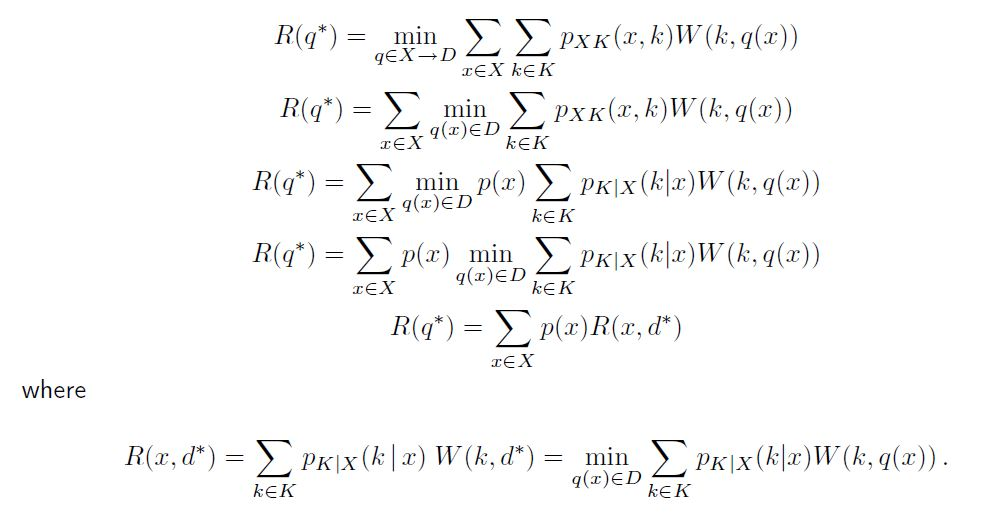
\includegraphics[width=12cm]{bayesian_risk.jpg}
\caption{Bayesovský risk}
\label{fig:bayes}
\end{center}
\end{figure}

\begin{figure}[h]
\begin{center}
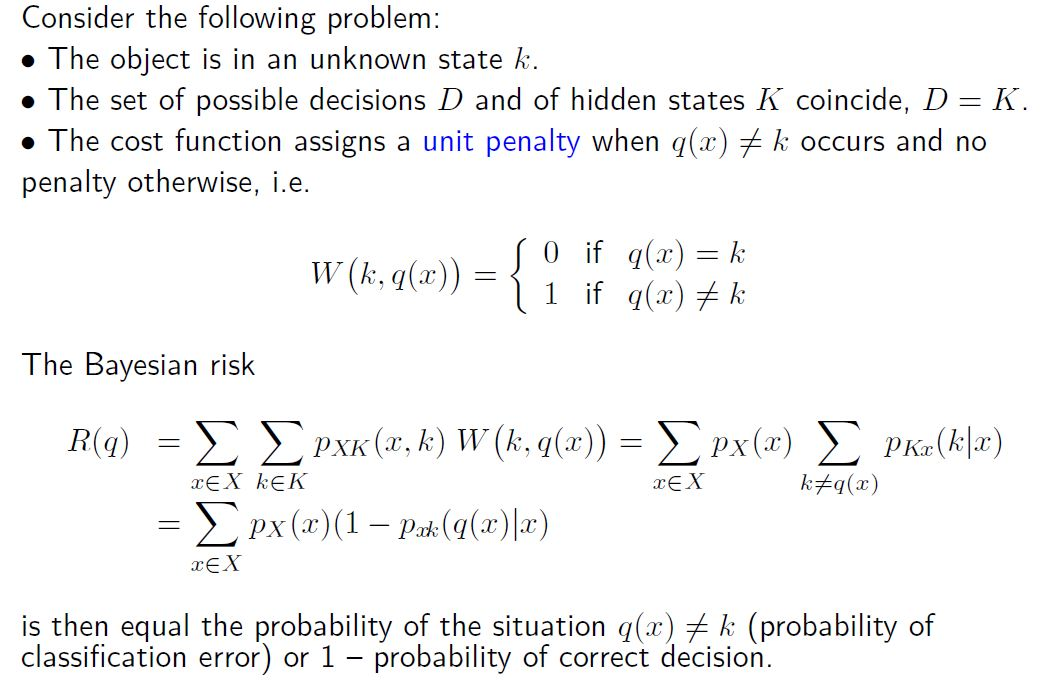
\includegraphics[width=12cm]{bayes_example.jpg}
\caption{Bayesovský risk příklad 1}
\label{fig:bayes_example1}
\end{center}
\end{figure}

\begin{figure}[h]
\begin{center}
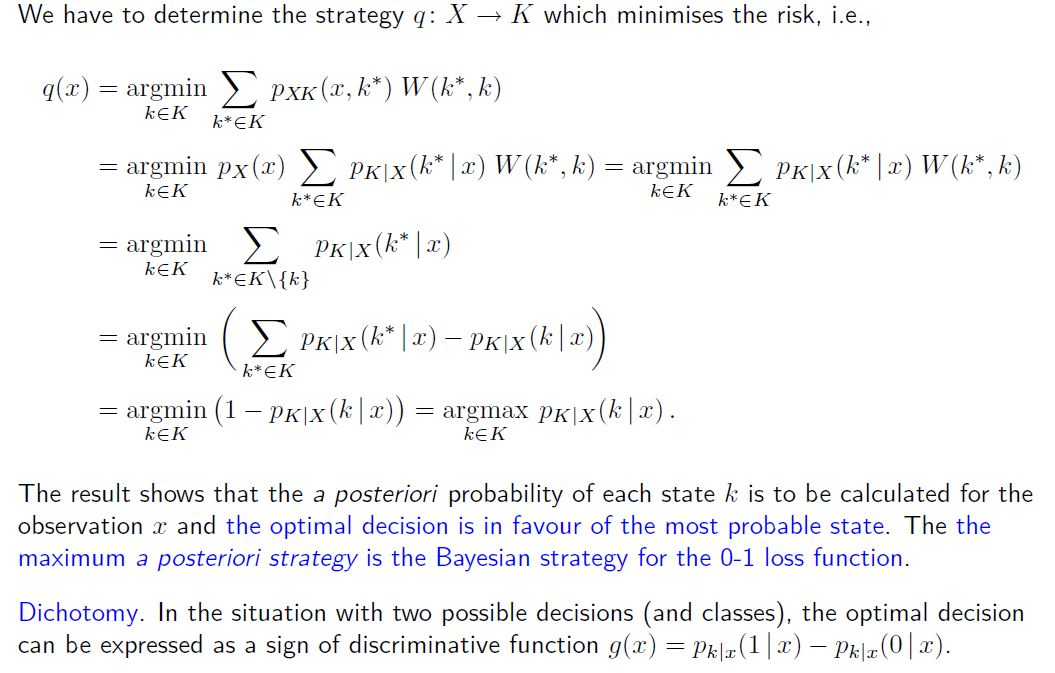
\includegraphics[width=12cm]{bayes_example1.jpg}
\caption{Bayesovský risk příklad 2}
\label{fig:bayes_example2}
\end{center}
\end{figure}

\begin{figure}[h]
\begin{center}
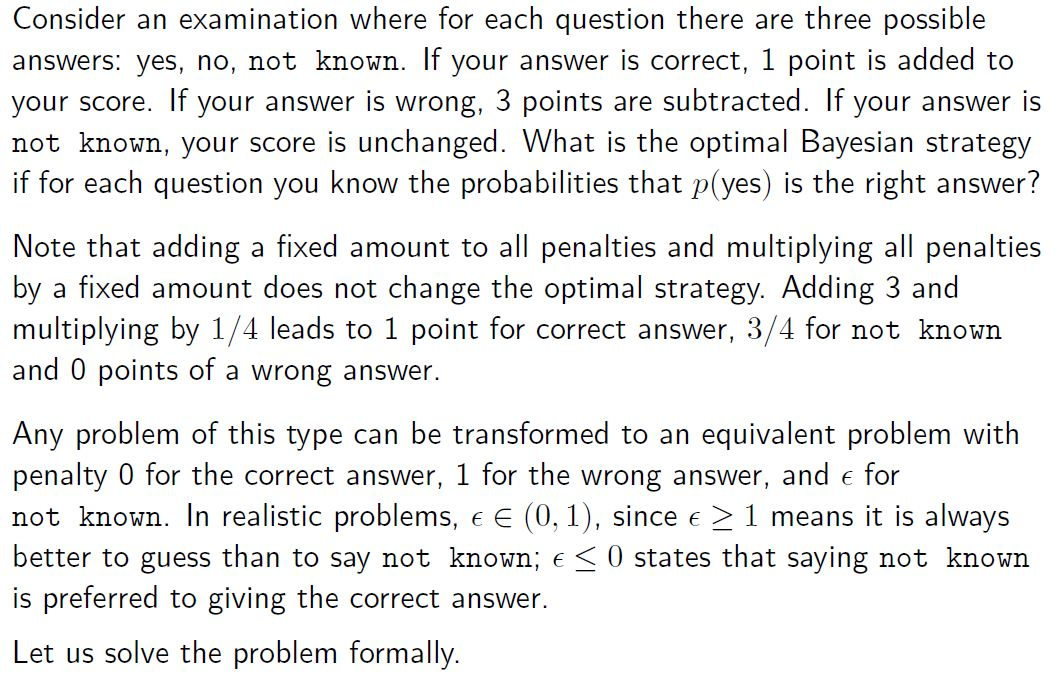
\includegraphics[width=12cm]{bayes_reject_example.jpg}
\caption{Bayesovský risk s nevím příklad 1}
\label{fig:bayes_reject_example1}
\end{center}
\end{figure}

\begin{figure}[h]
\begin{center}
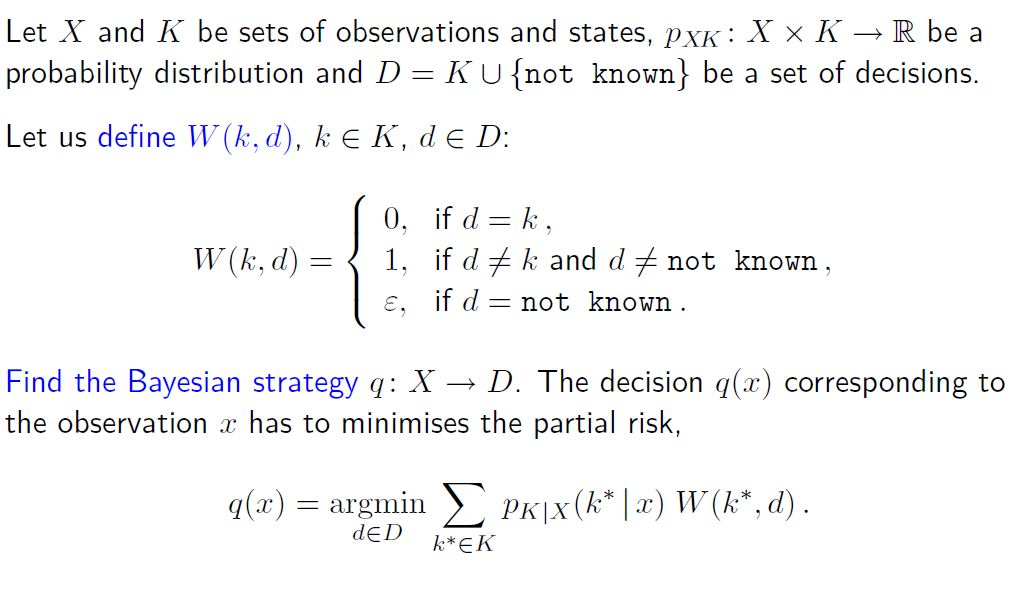
\includegraphics[width=12cm]{bayes_reject_example1.jpg}
\caption{Bayesovský risk s nevím příklad 2}
\label{fig:bayes_reject_example2}
\end{center}
\end{figure}

\begin{figure}[h]
\begin{center}
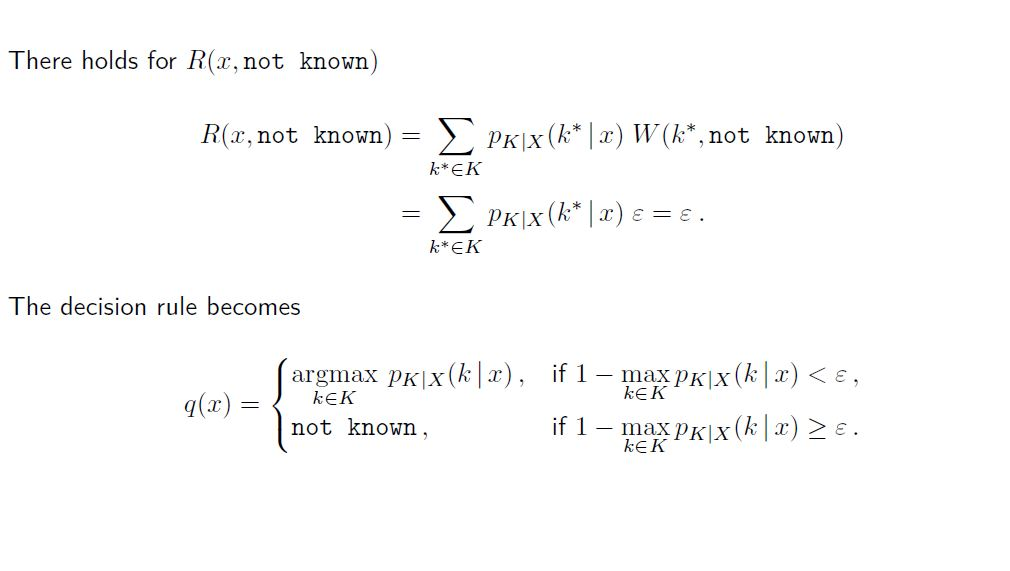
\includegraphics[width=12cm]{bayes_reject_example2.jpg}
\caption{Bayesovský risk s nevím příklad 3}
\label{fig:bayes_reject_example3}
\end{center}
\end{figure}

\section{Nebayesovské rozhodování}

V situacích kdy neznáme apriorní pravděpodobnosti (např protože k není náhodný jev) nebo nemůžeme porovnávat ztrátu pro různé situace.

\subsection{Neyman-Pearson}

Předpokládejme dva stavy $k = 1$ bezpečný a $k = 2$ nepezpečný. Náš úkol je rozdělit množinu pozorování $X$ na množinu $X_1$ bezpečných stavů a množinu $X_2$ nebezpečných stavů takových že $X_1 \cup X_2 = X$ a $X_1 \cap X_2 = \emptyset$. $p_{X|K}(x|k)$ jsou známé. Strategie je charakterizována dvěmi čísly. Přehlédnuté nebezpečí(overlooked danger) $\displaystyle\sum_{x \in X_2}p_{X|K}(x|1)$ a planý poplach(false alarm) $\displaystyle\sum_{x \in X_1}p_{X|K}(x|2)$. Hlavní myšlenka tohoto rozhodování je minimalizace false alarm, za předpokladu že overlooked danger je menší než $\epsilon$.

\subsection{Minimax}

Minimax minimalizuje nejhorší možnou chybu vzhledem k neznámým apriorním pravděpodobnostem, což pro rozhodování mezi 2mi stavy odpovídá minimalizaci $argmin_{d(x)}\max\{\int_{X_2}p(x|1)dx, \int_{X_1}p(x|2)dx\}$. Risk minimaxního rozhodování není nikdy menší než risk bayesovského rozhodování pro nejnepříznivější apriorní pravděpodobnosti.

\end{document}